Though the line-integrated metastable densities are one of only a few
measurements made in the development of the \acs{rpnd}, they only provide a
limited view of what is happening. In addition to the metastables are ions,
electrons, a vast array of other excited states, and the electric fields. In an
effort to expand on the details of what is occurring within the \acs{rpnd}, it
is desirable to develop a model which can infer other properties from the
metastable measurements. This is possible, because the electrons which gain
energy from the electric fields are responsible for the excitation of the
metastables, other atomic states, and ions. The ideal model would solve the
Boltzmann equation (equation~\ref{eq:boltzmann}) for each species, over the
entire geometry, in all dimensions, for as long as was required to reach
equilibrium.

Unfortunately, these requirements are somewhat problematic. Solutions to the
Boltzmann equation alone are difficult \cite{Lieberman2005}, let alone for the
dozens of species which may be present in the \acs{rpnd}. The spatial
discretization can be estimated as the cube of the largest length scale (the
discharge apparatus length, about 30 cm) divided by the smallest length scale
(on the order of the Debye length, about 20 $\mu$m). This approximation suggests
the need for $2\times10^{12}$ spatial cells. Similar calculations can be made
for the time (from nanoseconds to minutes) and velocity (from thermal to 100s of
eV) scales. It is immediately apparent that a numerical system of this size
would exceed the capabilities of any existing computer.

\section{Model Development}

Therefore, some approximations of the Boltzmann equation were required in order
to obtain a computationally tractable problem. As discussed in
Chapter~\ref{chp:theory}, the most common approach, and the one applied here, is
the use of \emph{moments} of the Boltzmann equation. These moments average out
the velocity dependence of the Boltzmann equation in favor of macroscopic
properties such as particle densities and mean velocities. They are often used
to develop various fluid approximations for plasmas \cite{Chen1984} (e.g.\ the
two fluid model, the magnetohydrodynamic equations, etc.). Solutions of
these fluid equations have been tremendously successful in the description of
everything from plasma display panels \cite{Rauf1999b} to interstellar plasmas
\cite{Linde1998}.

The use of moments of the Boltzmann equation does introduce some additional
problems. Reaction rates, such as ionization and excitation, are very sensitive
to changes in the distribution of particle velocities. This presents a problem
as the moments of the Boltzmann equation average out the velocity dependence.
Therefore, a distribution function must be assumed or calculated in order to
determine the reaction rates. The Maxwell-Boltzmann and Druyvesteyn
distributions from Chapter~\ref{chp:theory} are often used for this purpose.
However, they require a number of assumptions which are not necessarily true for
most plasmas. In cases when these distributions cannot be applied, approximate
solutions of the Boltzmann equation are often used \cite{Hagelaar2005} which
employ detailed reaction cross sections. The choice between the simple
equilibrium solutions and the more complex approximations is not easy as the
\acs{eedf} is rarely known \emph{a priori}. This topic is considered more
thoroughly in section~\ref{sec:dists}.

From another perspective, fluid models in multiple dimensions are still
computationally expensive. In large geometries, this can limit the number of
species and reactions which can be considered by the simulation
\cite{Lieberman2005}. For this reason, simulations often limit themselves to one
or a few excited states, preventing detailed comparisons to spectroscopic data.
However, such comparisons can reveal information about the degree of equilibrium
in the plasma and the electron temperatures, both of interest in the \acs{rpnd}.
Therefore, additional simplifications were necessary in order include additional
excited states.

As simplifications had already been made to the velocity space, the choice was
between reduced temporal resolution and reduced spatial resolution. A reduction
in temporal resolution was unreasonable given the fixed duration of the pulse
and its afterglow. In contrast, the metastable measurements were already made on
small spatial scale relative to the metastable gradients seen in
Chapter~\ref{chp:metastables}. Therefore, the spatial dependence was eliminated
to produce what is known as a ``global model.'' The final model tracked a total
of 32 different excited states of helium from before the pulse until the return
of the first reflection.

In order to compare the metastable measurements to the global results, it was
necessary to convert the line-integrated densities to densities along the path
of the laser. It has been noted that a similar \acs{fiw} \cite{Vasilyak1994} and
the same \acs{rpnd} \cite{Weatherford2012} exhibit radial variations in emission
intensity, electron density, and metastable density. Unfortunately, the cause of
this is not clearly understood, though it has been suggested that high-energy
electrons from the walls may be responsible \cite{Weatherford2012a}. Lacking any
empirical, theoretical, or numerical results which describe the evolution of the
radial profile during the discharge, it was necessary to assume one. In this
report, the plasma was assumed to be uniform across the diameter of the
discharge. This assumption likely affects the inferred plasma parameters,
however more accurate results are possible provided time-resolved measurements
of the radial metastable density or an improved understanding of the \acs{rpnd}.

\subsection{Continuity Equation}

The equation~\ref{eq:cont}, the continuity equation, forms the basis for
tracking the populations of the excited states in the plasma. Having assumed
that the spatial variations are zero, the equation reduces to,
\begin{equation}
  \frac{d n_\alpha}{dt} = G_\alpha - L_\alpha,
  \label{eq:zdmcont}
\end{equation}
where $\alpha$ identifies the particle species, $G$ is the gain term, and $L$ is
the loss term. The gain and loss terms represent all possible reactions which
can alter the population of the species under consideration. In the presented
model, only helium, excited helium states, helium ions, and electrons were
treated. Also present, to some degree, were gaseous impurities and helium
dimers. As observed in Chapter~\ref{chp:metastables}, the combined effects of
these species on the metastable densities took place with an e-folding time of
about 25 $\mu$s. As the simulations are limited to the period of time before the
first reflection arrives (140 ns), these species were neglected in the model.

There were several possible processes that were considered for inclusion in the
model:
\begin{itemize}
  \singlespacing
  \item electron impact ionization,
  \item electron impact (de)excitation,
  \item atomic impact (de)excitation,
  \item atomic excitation transfer,
  \item dielectronic recombination,
  \item three-body recombination,
  \item radiative decay, and
  \item diffusion.
\end{itemize}
As with the impurities and dimer formation, diffusion occurs on a much longer
time scale, and was subsequently neglected. Three-body recombination in the
volume of the discharge is not important at the estimated temperatures and
densities \cite{Lieberman2005}, therefore this too was neglected. In general,
dielectronic recombination is a rare process \cite{Nahar2010}, however it was
incorporated during early versions and was retained through the final revision.
Inter-atomic excitation and de-excitation is not generally considered important
given the low energies of the atoms in discharges.

The remaining processes were found to be the most important for the \acs{rpnd}.
This included electron-impact ionization and excitation which were, by far, the
most significant. In addition, excitation transfer between atoms was found to
occur at relevant rates \cite{Lieberman2005}. Finally, radiative decay between
states was included as this allowed the prediction of plasma emissions as well
as the cascade of excited states down to the metastable level.

Given these processes, equation~\ref{eq:zdmcont} was rewritten as,
\begin{multline}
  \frac{dN_i}{dt} =   n_e \left[       \sum_{j\neq i} N_j K^e_{j,i}(T_e) 
                                 - N_i \sum_{j\neq i}     K^e_{i,j}(T_e) \right]
                        + \left[       \sum_{j > i}   N_j K^o_{j,i} 
                                 - N_i \sum_{j < i}       K^o_{i,j}      \right] \\
                    + N_g \left[       \sum_{j\neq i} N_j K^a_{j,i} 
                                 - N_i \sum_{j\neq i}     K^a_{i,j}      \right].
  \label{eq:gcont}
\end{multline}
Here, the subscripts of $i$ and $j$ represent states of helium, $N$ is the state
density, $K$ is a rate coefficient, $T_e$ is the electron temperature, and $N_g$
is the neutral helium density. The first subscript of the rate coefficients
represents the initial excited state while the second coefficient represents the
final excited state. Therefore, $K_{ij}$ represents a process that transfers an 
atom from state $i$ to state $j$.

This equation is split into three sets of processes, represented by the
superscripts of the rate coefficients: $e$ - electron impact processes, $o$ -
radiative decay, and $a$ - atomic excitation transfer. The first bracketed term
on the right hand side contains all the rate coefficients for electron impact
excitation and de-excitation, including ionization processes. The second
bracketed term contains the rate coefficients for optical transitions in and out
of the excited state. The final bracketed term contains the gains and losses as
a result of excitation transfer caused by collisions with the ground state.
Collisions between excited states are neglected as their low densities result in
small reaction rates.

The rate coefficients in equation~\ref{eq:gcont} are compiled from a number of
different sources. This is particularly straight forward in the case of the
optical and atomic transitions, as neither features any dependence on the
\acs{eedf}. The optical transition rates and the energies of each level were
obtained from the NIST Atomic Spectra Database \cite{Kramida2012}. The
excitation transfer rate coefficients came from the studies of Catherinot and
Dubreuil \cite{Catherinot1981, Dubreuil1980}. These coefficients only covered
the transitions of $\Delta n=0$ for $n=3,4$ and no constants were found for
other $n$ or $\Delta n\neq 0$. Dielectronic recombination rates were adapted
from the work of Nahar \cite{Nahar2010}.

As for the electron-impact processes, the semi-empirical relations derived by
Ralchenko et al. \cite{Ralchenko2008} were used to calculate the electron
(de)excitation and ionization cross sections for levels through $n=4$. These
represented the most accurate set of cross sections available for neutral helium
and have a quoted accuracy of 10-30\% for $\Delta S=0$, and $>30$\% for $\Delta
S \neq 0$. Only the inelastic cross sections for collisions which increased the
energy of the excited state were provided. The inverse or superelastic cross
sections were calculated using the principle of detailed balance
\cite{Kunze2009},
\begin{equation}
  \sigma_{ji}(\epsilon) = \frac{\epsilon}{\epsilon - \Delta\epsilon_{ij}}
    \frac{g_j^2}{g_i}\sigma_{ij},
\end{equation}
where $\Delta\epsilon$ is the threshold energy of the $ij$ reaction and $g$ is
the statistical degeneracy of the corresponding state. These cross sections can
be used to calculate the rate coefficients for each reaction using
equation~\ref{eq:rate}. However, this leads back to the question of which
\acs{eedf} is appropriate for the \acs{rpnd}.

\subsection{Distribution Effects}\label{sec:dists}

Per the discussion of the Boltzmann equation in Chapter~\ref{chp:theory}, there
are two analytic equilibrium solutions: the Maxwell-Boltzmann distribution, and
the Druyvesteyn distribution. However, research by Starikovskaia and
Starikovskii \cite{Starikovskaia2001} has shown that the \acs{eedf} in a
nitrogen \acs{fiw} can deviate from both. Such a result is not too surprising
given the non-equilibrium nature of the \acs{fiw} discharge. Since the
\acs{rpnd} shares many of these same properties, it is possible that the
equilibrium solutions do not apply to the \acs{rpnd} either.

In order to better understand how the energy distributions may behave in a
\acs{rpnd}, a numerical study of the \acs{eedf} in a helium \acs{rpnd} was
conducted. First, a particle-in-cell (\acs{pic}) code was used to simulate the
effect of a voltage pulse on electrons in a quasi zero-dimensional geometry.
This generated the evolution of the \acs{eedf} in a helium plasma as a function
of time. Then, the mean energy for the \acs{eedf} at each time was calculated.
This was then used to generate similar equivalent Maxwell-Boltzmann
distributions and solutions of the Boltzmann equation.

The \acs{pic} simulations do not attempt to solve the Boltzmann equation
directly. Instead, they simulate the behavior of many plasma particles in an
experimental geometry using the basic laws of motion and electromagnetism
\cite{Birdsall1991}. A discrete \acs{eedf} can then be calculated from the
particle population (or subset thereof). As the number of simulated particles
increases the discrete \acs{eedf} will approach the continuous \acs{eedf} which
would result from a solution of the Boltzmann equation.

Generally, \acs{pic} simulations do not make a one-to-one correspondence between
computer particles and physical particles--most plasma involve more particles
than can be reasonably simulated. Instead, they consider a population of
macro-particles, each of which possesses some statistical weight
\cite{Birdsall1991}. This weight allows the macro-particle to represent a group
of physical particles. 

The process by which the \acs{pic} simulation is conducted is illustrated in
figure~\ref{fig:pic}.
\begin{figure}
  \centering
  \setlength{\unitlength}{4.8in}
\begin{picture}(1.0, 0.5)
   \put(0.10, 0.35){\framebox(0.35, 0.10){\parbox{0.35\unitlength}{\footnotesize\centering Integration of equations \\ of motion, moving particles \\ $\vec{F}_i \rightarrow \vec{v}'_i \rightarrow x_i$}}}
   \put(0.45, 0.40){\line( 1,  0){0.10}}
   \put(0.55, 0.35){\framebox(0.35, 0.10){\parbox{0.35\unitlength}{\footnotesize\centering Particle loss/gain \\ at the boundaries \\ (emission, absorption, etc.)}}}
   \put(0.90, 0.40){\line( 1,  0){0.05}}
   \put(0.95, 0.40){\line( 0, -1){0.10}}
   \put(0.70, 0.20){\framebox(0.30, 0.10){\parbox{0.30\unitlength}{\footnotesize\centering Monte Carlo collisions \\ $\vec{v}'_i \rightarrow \vec{v}_i$}}}
   \put(0.95, 0.20){\line( 0, -1){0.10}}
   \put(0.95, 0.10){\line(-1,  0){0.10}}
   \put(0.60, 0.05){\framebox(0.25, 0.10){\parbox{0.25\unitlength}{\footnotesize\centering Weighting \\ $(x,\vec{v})_i \rightarrow (\rho, \vec{J})_j$}}}
   \put(0.60, 0.10){\line(-1,  0){0.20}}
   \put(0.15, 0.05){\framebox(0.25, 0.10){\parbox{0.25\unitlength}{\footnotesize\centering Integration of field \\ equations on grid \\ $(\rho, \vec{J})_j \rightarrow (\vec{E},\vec{B})_j$}}}
   \put(0.15, 0.10){\line(-1, 0){0.10}}
   \put(0.05, 0.10){\line( 0, 1){0.10}}
   \put(0.00, 0.20){\framebox(0.20, 0.10){\parbox{0.20\unitlength}{\footnotesize\centering Weighting \\ $(\vec{E},\vec{B})_j \rightarrow \vec{F}_i$}}}
   \put(0.05, 0.30){\line( 0,  1){0.10}}
   \put(0.05, 0.40){\line( 1,  0){0.05}}
   \put(0.46, 0.22){\Huge $\circlearrowright$}
   \put(0.4725, 0.2275){\footnotesize\centering $\Delta t$}
\end{picture}

  \caption{Schematic description of the \acs{pic} simulation process, adapted
    from \cite{Birdsall1991}.}
  \label{fig:pic}
\end{figure}
The process begins with the definition of a system geometry and an applied
electromagnetic field, $\vec{E}$ and $\vec{B}$. In this case, the system is
strictly one-dimensional, so each macro-particle only possess one spatial
component, $x$. However, to account for magnetic field effects, each
macro-particles possesses three velocity components, $\vec{v}$. This is followed
by an initialization of the particle positions and velocities. The number of
particles and the their positions are usually chosen to given a specific plasma
density, and the velocities are often chosen to represent some initial
distribution of energy. The Lorentz equation, $\vec{F} = q(\vec{E} +
\vec{v}\times\vec{B})$, is then used to push each particle to a new position for
a given time step, $\Delta t$. Particles born or lost at the boundaries are then
accounted for. This is followed by a modeling of collisions (including
ionization and excitation) using Monte Carlo techniques \cite{Birdsall1991}. The
charges of the macro-particles are then weighted to a spatial grid, and the
fields are recalculated, and the next time step begins.

The XPDP1 code, developed by Verboncoeur et al. \cite{Verboncoeur1993}, was used
to conduct the \acs{pic} simulations. The code was originally designed to
simulate a one-dimensional discharge between two parallel electrodes. However,
the electrodes complicate the study of the \acs{eedf}. Charged particle
collection near the boundaries will introduce spatial variations in the
\acs{eedf}. In addition, such collection can lead to large regions of space
charge which can shield out the applied electric field. In order to address
these issues, the code was modified to use periodic boundary conditions. Such
conditions result in a quasi zero-dimensional simulation, equivalent to a plasma
of infinite extent. This eliminates the issue of spatial variations in the
\acs{eedf}.

Previous measurements of the electric field in a similar \acs{fiw} suggested
that the electric field values varied from 0-350 Td \cite{Takashima2011}. Based
on this, it was decided to examine the distribution characteristics from 10-600
Td. This range should be adequate to cover all conditions within the \acs{rpnd}
in question. The background gas was helium at a pressure of 2.0 Torr. The
initial plasma was assumed to be quasineutral with a density of
$1.0\times10^{8}$ cm$^{-3}$ and 10$^4$ macro-particles. Electrons were
initialized with a thermal energy of 2.0 eV, and the helium ions were given an
initial energy of 0.025 eV. 

The internal set of cross sections, which include elastic scattering,
excitation, and charge exchange were used. The cross sections have a
semi-empirical form which increases linearly with energy to a peak value after
which it declines as the logarithm of the energy, divided by the energy. The
time domain of the simulation was 10 ns, approximately the time required for the
\acs{eedf} to reach equilibrium with the applied field. The distributions from
the \acs{pic} simulations were sampled every 0.25 ns. The spatial domain was
discretized at 1 $\mu$m intervals over a total domain of 10 cm. Based on the
highest energy electrons in the system, a time step of $4\times10^{-13}$ s was
chosen in order to satisfy the Courant-Friedrich-Lewy stability condition.

BOLSIG+ was used to obtain the approximate solutions of the Boltzmann equation
\cite{Hagelaar2005}. This is a publicly available computer code which uses the
two-term expansion of the Boltzmann equation to solve for the \acs{eedf} for a
given electric field. In this approach, Legendre polynomials are used to expand
the \acs{eedf} into an equilibrium solution and a relatively small
non-equilibrium component. This implied assumption, that the distribution is
accurately represented by a small perturbation superimposed on an equilibrium
solution, puts constraints on the magnitude of the reduced electric field. In
the case of BOLSIG+, the solver fails to converge for fields approaching 1000
Td.

The solver was inititialized with the cross sections for helium generated by
Alves and Ferreira \cite{Alves2013}. The temporal growth model for electrons was
used, and the electron-electron collisions were not neglected as a result of the
low ionization fraction in the \acs{rpnd}. Solutions were calculated for a range
of electric fields and then tabulated according to their mean energy. A nearest
neighbor interpolation scheme was used to generate an \acs{eedf} for the mean
energies from the \acs{pic} simulations.

These same energies were used to determine equivalent Maxwell-Boltzmann
distributions for comparison. The results of these calculations can be seen in
figure~\ref{fig:picmb},
\begin{figure}
  \centering
  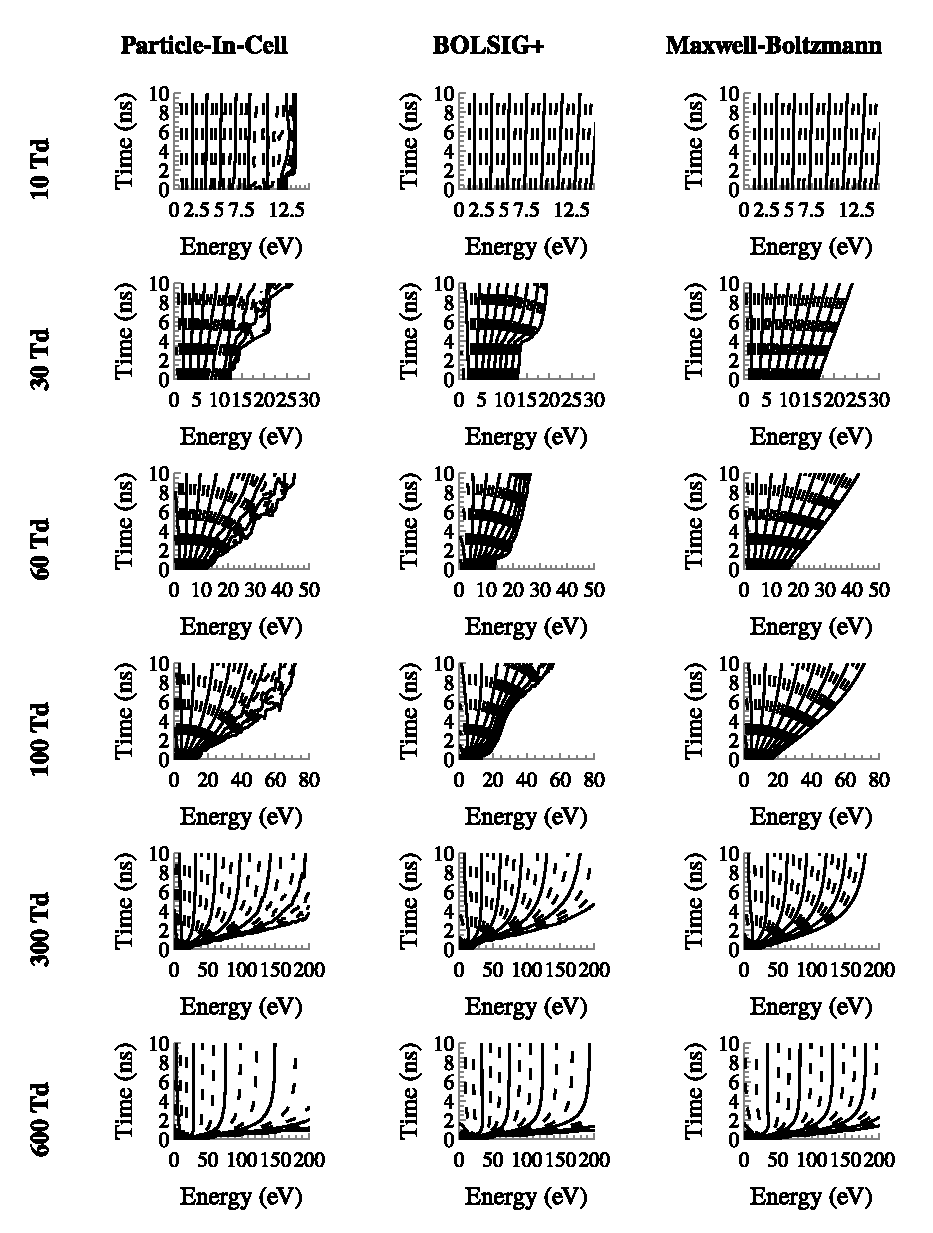
\includegraphics{./chapters/modeling/figures/picmb.eps}
  \caption{Contour plots of the \acs{eedf}s determined from \acs{pic}
    simulations, and the corresponding Maxwell-Boltmzann distributions for a range
    of electric fields.}
  \label{fig:picmb}
\end{figure}
as a series of contour plots comparing the results for each approach. The
jaggedness of the \acs{pic} simulations results from the finite number of
particles in the system and the low probability of high energy electrons. This
problem is ameliorated at higher electric fields where the probability of
high-energy electrons increases. An increase in the number of electron
macro-particles, resulting from ionization, also helps to reduce this effect.

At 10 Td, the \acs{eedf}s are relatively unchanged over the duration of the
simulation. The subtle slopes of the contours suggest a small increase in the
overall temperature and energy of the system. The rate of increase in
temperature increases as the value of the electric field is increased. At 30 Td,
the contours of each approach are essentially linear with similar slopes. The
only noticeable deviation is the closer spacing of the contours from BOLSIG+.
Thus the probability distribution falls off faster with energy for this case
relative to the \acs{pic} simulations and the corresponding Maxwell-Boltzmann
distributions.

At 60 and 100 Td, the \acs{pic} results and Maxwell-Boltzmann distributions
continue to feature contour spacings which increase linearly with time. In
contrast, the BOLSIG+ solutions have contour spacings which are monotonically
increasing, but at a rate which varies in time. Additionally, the spacing
between the various levels is less consistent than for the \acs{pic} simulations
or the Maxwell-Boltzmann distributions. By the end of the simulation period, the
overall width of BOLSIG+ contours is less than either of the other approaches.

However, by 300 and 600 Td the situation has slight changed. The
Maxwell-Boltzmann distributions show consistently less breadth than the
\acs{pic} results of the BOLSIG+ solutions. Close examination shows that the
\acs{pic} simulations have larger populations of low energy (less than 20 eV)
and high energy (greater than 100 eV) electrons. This can be traced back to the
form of the helium cross sections used in XPDP1. The only reactions available to
electrons in the simulation are elastic scattering, excitation (19.6 eV
threshold), and ionization (24.6 eV threshold). Thus the electron population is
depleted at values above around 20 eV, as a result of these inelastic processes.
Likewise, the electron population begins to rebound at higher energies as the
inelastic processes turn off. The Maxwell-Boltzmann solutions are quite simple
and do not account for the variation of the cross sections with respect to
energy. This explains the increased consistency of the \acs{pic} and BOLSIG+
results at high electric field values.

Generally, the Maxwell-Boltzmann results appear to provide the best match to the
\acs{pic} simulations at electric fields of 100 Td and below. At higher fields,
the BOLSIG+ results provide a better approximation of the \acs{pic} results.
If the electric fields measured by Takashima et al.\ are the same as those in the
\acs{rpnd} studied here, then the Boltzmann solver would be the best choice at
the peak field values. However, for a very large fraction of the time, the
Maxwell-Boltzmann distribution would appear to provide the best approximation of
the electron distributions in the system. As a result, it was decided to use
this distribution for the development of the global model.

\subsection{Energy Equation}

Given a form for the distribution function, it is now possible to calculate the
rate coefficients in equation~\ref{eq:gcont} at each time step. However, as was
seen in figure~\ref{fig:picmb}, the distribution function changes over time. In
that case, the \acs{pic} simulations were used to calculate the mean electron
energy which, in turn, was used to determine the appropriate Maxwell-Boltzmann
distribution. However, as of yet, no mechanism has been provided to evolve the
mean electron energy in the absence of such simulations.

With suitable assumptions, equation~\ref{eq:energy} (the second moment of the
Boltzmann equation) can provide the means to evolve the mean energy with each
time step. Given the assumptions underlying the global model, the spatial
derivatives can be neglected so that
\begin{equation}
  \frac{d}{dt}\left(\frac{3}{2}p_e\right) =
  \frac{d}{dt}\left(\frac{3}{2}p_e\right)\bigg|_\mathrm{coll}.
\end{equation}
Using the isothermal equation of state, $p=n\kB T$, this can be rewritten as,
\begin{equation}
  \frac{d}{dt}\left(\frac{3}{2}n_e\kB T_e \right) =
  \frac{d}{dt}\left(\frac{3}{2}n_e\kB T_e \right)\bigg|_\mathrm{coll}.
  \label{eq:energy2}
\end{equation}
The term on the RHS is the collision operator which expresses energy gained or
lost by electrons\footnote{In some plasmas, it is desirable to also treat gas
heating with a similar equation as it can have an appreciable impact on certain
rate constants. However, as noted in Chapter~\ref{chp:metastables}, the gas
temperature of the \acs{rpdn} in question remains at room temperature.} in
particle collisions.

Several different forms of particles collisions must be considered by the global
model. Once the electron population surpasses the 19.6 eV threshold, a great
deal of energy will be exchanged with excited helium species through inelastic
collisions. In addition, the electron population will tend to thermalize with
the background gas over long periods of time via elastic collisions. Finally,
energy is gained by the electrons through the applied electric field. Together,
these phenomena replace the term on the RHS of equation~\ref{eq:energy2} with,
\begin{equation}
  \frac{e^2n_eE(t)^2}{m_ek_m(T_e)N_g}
  - n_ek_m(T_e)N_g\left(\frac{3m_e}{M}\right)\frac{3}{2}\kB(T_e-T_g)
  - n_e \sum_i \sum_{j\neq i} K^e_{ij}N_i\Delta\epsilon_{ij},
  \label{eq:energyparts}
\end{equation}
where $E(t)$ is the time-varying electric field, $k_m$ is the electron momentum
transfer frequency from Pack et al. \cite{Pack1992}, and $\Delta\epsilon_{ij}$
is the energy lost or gained by the electron in atomic (de)excitation reactions.
The first term includes the DC conductivity \cite{Lieberman2005} of the plasma,
and accounts for the heating of the electrons by the electric field. The second
term is the elastic cooling of the electrons by the neutral atoms, where the gas
temperature is assumed fixed. The third term is the energy gained or lost by the
electrons in atomic (de)excitation reactions. Equation~\ref{eq:energyparts},
with equations~\ref{eq:energy2} and~\ref{eq:gcont} are sufficient to solve for
the evolution of the electron temperatures, electron densities, excited state
densities, and plasma emissions as functions of time.

\subsection{Model Solutions}

Equation~\ref{eq:gcont} can be rewritten for each atomic state, $i$, resulting
in a set of linear, first order differential equations,
\begin{multline}
  \frac{d}{dt}
  \begin{pmatrix}
    N_1 \\
    N_2 \\
    \vdots \\
    N_M
  \end{pmatrix}
  = n_e
  \begin{pmatrix}
    -\sum_{j\neq 1}K^e_{1,j} & K^e_{2,1}      & \hdots & K^e_{M,1} \\
    K^e_{1,2}      & -\sum_{j\neq 2}K^e_{2,j} & \hdots & K^e_{M,2} \\
    \vdots         & \vdots         & \ddots & \vdots    \\
    K^e_{1,M}      & K^e_{2,M}      & \hdots & -\sum_{j\neq M}K^e_{M,j}
  \end{pmatrix}
  \cdot
  \begin{pmatrix}
    N_1 \\
    N_2 \\
    \vdots \\
    N_M
  \end{pmatrix} \\
  +
  \begin{pmatrix}
    0      & K^o_{2,1}              & \hdots & K^o_{M,1} \\
    0      & -\sum_{j < 2}K^e_{2,j} & \hdots & K^o_{M,2} \\
    \vdots & \vdots                 & \ddots & \vdots    \\
    0      & 0                      & \hdots & -\sum_{j < M}K^e_{M,j}
  \end{pmatrix}
  \cdot
  \begin{pmatrix}
    N_1 \\
    N_2 \\
    \vdots \\
    N_M
  \end{pmatrix} \\
  + N_g
  \begin{pmatrix}
    -\sum_{j\neq 1}K^a_{1,j} & K^a_{2,1}      & \hdots & K^a_{M,1} \\
    K^a_{1,2}      & -\sum_{j\neq 2}K^a_{2,j} & \hdots & K^a_{M,2} \\
    \vdots         & \vdots         & \ddots & \vdots    \\
    K^a_{1,M}      & K^a_{2,M}      & \hdots & -\sum_{j\neq M}K^a_{M,j}
  \end{pmatrix}
  \cdot
  \begin{pmatrix}
    N_1 \\
    N_2 \\
    \vdots \\
    N_M
  \end{pmatrix}, \\
\end{multline}
where $M$ is the total number of atomic states and $\epsilon_i <
\epsilon_{i+1}$. An additional equation can be added to separately account for
electrons as well as electron-specific processes, however the model assumed
quasineutrality by enforcing the relation $N_{ion}=n_e$. Changes in the density
of each atomic state were calculated by numerical integration of these
equations. The range of time scales exhibited by the \acs{rpnd} made it
desirable to implement adaptive control of the time step size. For this reason,
the Runge-Kutta-Fehlberg method, adapted from Bradie \cite{Bradie2006}, was
used.

Initial metastable densities were determined from the \acs{las} measurements.
Initial electron densities were determined from \acs{lcif} measurements made by
Weatherford \cite{Weatherford2012a}. However, these measurements were only
available for 1.0, 4.0, and 8.0 Torr. Previous studies have found that initial
electron density can have a significant effect on the parameters of a helium
\acs{fiw} \cite{Takashima2011}, therefore subsequent simulations were limited to
the three conditions for which electron density measurements were available.

No electron temperature measurements were possible at the low densities in the
pre-pulse period, therefore a temperature of 0.2 eV was assumed. This
temperature was used to generate the equilibrium excited state densities for
non-metastable states. As the \acs{las} measurements showed no appreciable
change in gas temperature, the neutral gas temperature was fixed at 300 K for
the duration of the simulation.  

Though the applied potential is well known, the actual form of $E(t)$ is
significantly less clear. Again, \acs{fiw} measurements such as those performed
by Takashima et al. \cite{Takashima2011}, as well as the \acs{rpnd} measurements
of Ito et al. \cite{Ito2010}, and M\"{u}ller \cite{Muller2011a} provide some
idea of what to expect. Each study measured a Gaussian-like peak as the wave
crossed the measurement point. In the quiescent period following the wave, a
relatively small background electric field persisted, with a magnitude on the
order of 20-25\% of the of the wave. The duration and magnitude of this
persistent field varied substantially between studies. Given the indeterminate
value of this persistent field, the following simulations assumed a single
Gaussian pulse for the form of the electric field. The time domain of the
simulation was 190 ns, with the peak of the electric field pulse at 40 ns.

\section{Perturbation Study}

The global model simulations depended, to a large extent, on the initial
conditions of the system. Without a clear process by which to calculate the
error in the results of the simulations, it was desirable to investigate the
sensitivity of the results to various factors. In order to examine these
effects, a preliminary fit was made to the 4.0 Torr measurements, and the
conditions of this fit were independently perturbed by $\pm10\%$. The conditions
studied were pressure, peak electric field, pulse-width, and initial electron
density.

The nominal conditions of the simulation are recorded in table~\ref{tbl:nominal}
\begin{table}
  \centering
  \caption{Nominal simulation parameters for the 4.0 Torr operating condition.}
  \begin{tabular}{llll}
    \toprule
    Pressure & Initial Electron    & Pulse      & Peak Electric \\
    (Torr)   & Density (m$^{-3}$)  & width (ns) & Field (Td)\\ 
    \midrule
    4.0      & 5.36$\times10^{13}$ & 40         & 207 \\
    \bottomrule
  \end{tabular}
  \label{tbl:nominal}
\end{table}
and results of these simulations are shown in figure~\ref{fig:perturbed}.
\begin{figure}
  \centering
  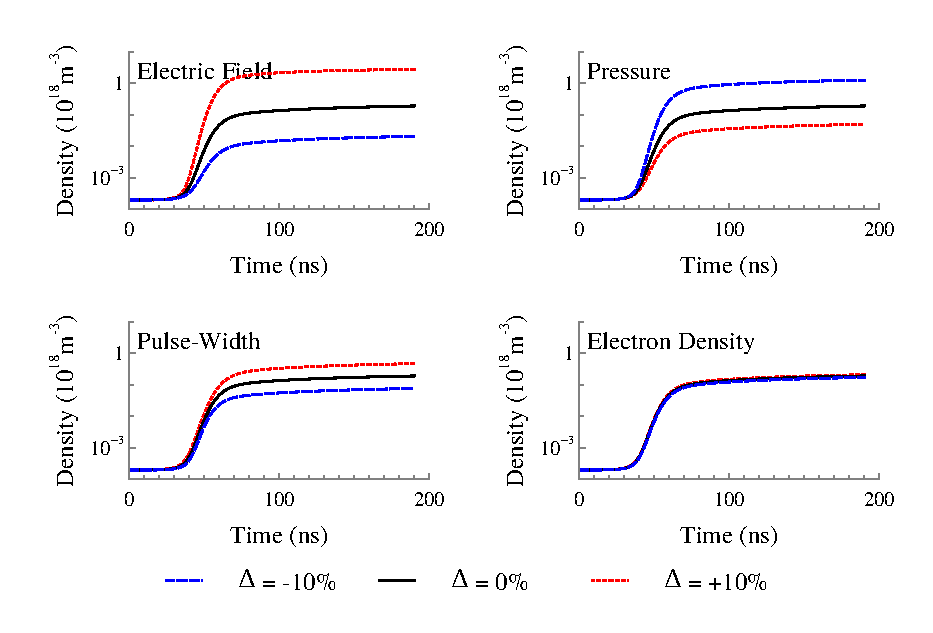
\includegraphics{./chapters/modeling/figures/perturbed.eps}
  \caption{Simulations showing the effects of perturbations to the initial
  conditions on the metastable dynamics.}
  \label{fig:perturbed}
\end{figure}
Based on the results of the global model, it is apparent that the initial
electron density has a relatively small impact on the metastable dynamics.
Closer examination of the results reveal that the final metastable densities
change by approximately $\pm10\%$ in concert with the perturbations to the
electron density. In contrast, changes to the pulse-width produce much more
significant changes in the metastable densities. As the pulse-width is
increased, the metastable densities increase. Knowing that the electric field is
fixed, this change can be attributed to the increase in energy deposited in the
electron population.

The two largest factors in the determination of the metastable densities were
the neutral gas pressure and the electric field. Small changes to either value
resulted in large changes in the metastable densities. As can be seen in
figure~\ref{fig:perturbed}, increases in pressure corresponded to a decrease in
metastable densities. Changes to the neutral gas pressure tend to affect the
system via several different mechanisms. As seen in
equation~\ref{eq:energyparts}, increases to the gas pressure tend to decrease
the energy deposited in the electrons, and increases losses due to elastic
scattering, thus reducing the energy that can be deposited in excited states.
This competes with the increased number of ground state atoms available for
excitation.

The significant impact of the electric field can be traced back to changes in
the ionization rate for each condition. As seen in figure~\ref{fig:ionrates},
\begin{figure}
  \centering
  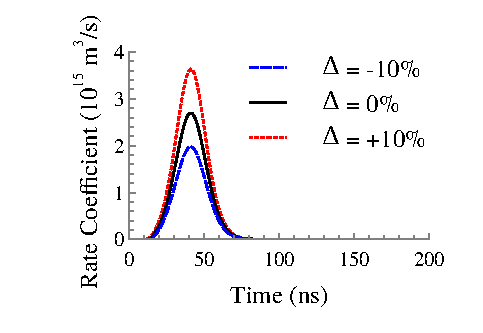
\includegraphics{./chapters/modeling/figures/ionrates.eps}
  \caption{Ionization rates coefficients corresponding to the perturbed electric
  field simulations.}
  \label{fig:ionrates}
\end{figure}
the magnitude of the ionization rate coefficient corresponds to the magnitude of
the electric field. While the changes are somewhat modest, as seen in
Chapter~\ref{chp:theory}, ionization processes are exponential with time. This
means that small changes to the rate coefficient manifest as large differences
in the final electron density. Since the rate of metastable generation is
proportional to the electron density, these changes to the electron density
equate to changes in the metastable density.

There is a high degree of confidence in the pressure measurements, therefore it
remained fixed throughout the simulations. Likewise, the initial electron
density measurements are considered reliable and remained fixed. As was
previously mentioned, the electric field is not well-known in the \acs{rpnd}
wave front. However, equally unknown is the pulse-width.

As a result,
the only parameters available to match the metastable dynamics were the electric
field and the pulse-widths. Unfortunately, there is no clear process by which to
adjust these values in order to obtain an optimal match to the metastable data.




\section{Plasma Dynamics}



\section{Summary}


